%=====================================================================
%  Advanced Optimization  --  Chapter 19  (12pt edition, v3)
%  Nocedal & Wright, Chapter 19: Interior-Point Methods for Nonlinear Programming
%  Centered on Sections 19.1--19.3. The course goes from Chapter 12 directly to
%  Chapter 19, so the tools of Chapters 15--18 that Chapter 19 uses are explained
%  where they first appear, marked "(From Chapter 15.)" etc.
%  Organized around what differs from a convex problem: the Newton step need not
%  be a descent direction (inertia), the KKT matrix can be singular, and steps
%  need an acceptance test (merit function, filter, restoration, SOC).
%  The last part maps the IPOPT iteration log to the symbols of the deck.
%
%  Layout rules for this deck (preamble copied from ch12v8.tex)
%   - body 12pt; nothing in the body below 10pt; footline 8pt
%   - one theorem per slide, or at most three displayed equations
%   - proofs are omitted; a red "Read:" pointer gives the pages in the book
%   - equation numbers and theorem statements follow the book
%   - material that is not in the book is marked "(Not in the book.)"
%   - figures are redrawn, not copied from the book
%   - no [shrink] option anywhere
%=====================================================================
\documentclass[aspectratio=169,12pt]{beamer}

\usetheme{default}
\usecolortheme{seahorse}
\useinnertheme{rectangles}
\setbeamersize{text margin left=7mm,text margin right=7mm}
\setbeamertemplate{navigation symbols}{}
\setbeamerfont{title}{series=\bfseries,size=\LARGE}
\setbeamerfont{subtitle}{size=\large}
\setbeamerfont{institute}{size=\small}
\setbeamerfont{frametitle}{series=\bfseries,size=\large}
\setbeamerfont{block title}{series=\bfseries,size=\normalsize}
\setbeamerfont{footline}{size=\scriptsize}   % 8pt at 12pt base
\setbeamercolor{frametitle}{fg=black!85,bg=black!5}
\setbeamercolor{block title}{bg=structure!25,fg=black!85}
\setbeamercolor{block body}{bg=structure!8}
\setbeamercolor{alerted text}{fg=red!65!black}
\setbeamercolor{footline}{fg=black!60}
\setbeamertemplate{itemize item}{\small$\blacktriangleright$}
\setbeamertemplate{itemize subitem}{\footnotesize$-$}
\setbeamertemplate{enumerate items}[default]
\setbeamerfont{enumerate item}{size=\normalsize,series=\bfseries}
\setbeamertemplate{footline}{%
  \leavevmode\hbox to\paperwidth{\hskip7mm\usebeamerfont{footline}\usebeamercolor[fg]{footline}%
  \insertsection\hfill\insertframenumber\,/\,\inserttotalframenumber\hskip7mm}\vskip2.2mm}

\usepackage{amsmath,amssymb}
\usepackage{booktabs}
\usepackage{tikz}
% no math subscript below 8pt, also inside \small and \footnotesize text
\DeclareMathSizes{12}{12}{8}{8}
\DeclareMathSizes{10.95}{10.95}{8}{8}
\DeclareMathSizes{10}{10}{8}{8}

\newcommand{\R}{\mathbb{R}}
\newcommand{\xs}{x^{*}}
\newcommand{\gradf}{\nabla f}
\newcommand{\hessf}{\nabla^{2} f}
\newcommand{\la}{\leftarrow}
\newcommand{\eqn}[1]{\text{\small(#1)}}
% reading pointer to the book (page numbers: Nocedal & Wright, 2nd ed.)
\newcommand{\readbook}[1]{{\color{red}\textbf{Read:} #1}}
% marker for material that is not in the book
\newcommand{\notinbook}{{\small(Not in the book.)}}
% algorithm listing: statement | equation number
\newcommand{\algostretch}{1.12}
\newenvironment{algo}{\par\renewcommand{\arraystretch}{\algostretch}%
  \begin{tabular}{@{}l@{\hspace{2.2em}}l@{}}}{\end{tabular}\par}



% Chapter 19 notation (all as in the book)
\newcommand{\cA}{\mathcal{A}}
\newcommand{\cC}{\mathcal{C}}
\newcommand{\cE}{\mathcal{E}}
\newcommand{\cI}{\mathcal{I}}
\newcommand{\cL}{\mathcal{L}}
\newcommand{\hessL}{\nabla_{xx}^{2}\cL}
\newcommand{\Ae}{A_{\cE}}
\newcommand{\Ai}{A_{\cI}}
\newcommand{\cEx}{c_{\cE}(x)}
\newcommand{\cIx}{c_{\cI}(x)}
\newcommand{\rd}{\nabla f(x)-\Ae^{T}(x)y-\Ai^{T}(x)z}
\newcommand{\from}[1]{{\small(From #1.)}}
\usetikzlibrary{arrows.meta,patterns}
\tikzset{vec/.style={-{Stealth[length=2mm]},thick},
         lab/.style={font=\footnotesize,inner sep=1.5pt}}

\title{Advanced Optimization}
\subtitle{Chapter 19 --- Interior-Point Methods for Nonlinear Programming}
\author{Hongseok Kim}
\institute{Department of Electronic Engineering, Sogang University}
\date{Fall 2026}


\begin{document}

\section{Chapter 19: the problem}

\begin{frame}
  \titlepage
  \begin{center}\small
    Reading: Nocedal \& Wright, \emph{Numerical Optimization}, 2nd ed., Chapter 19
  \end{center}
\end{frame}

\begin{frame}{Why not guess the active set? Example 15.1 \from{Chapter 15}}
  If the active set were known, we would solve an equality-constrained problem.
  \[ \min\ \tfrac12(x-2)^{2}+\tfrac12(y-\tfrac12)^{2}\quad\text{s.t.}\quad
     (x+1)^{-1}-y-\tfrac14\ge 0,\ \ x\ge 0,\ \ y\ge 0 . \tag{15.5} \]
  Try each \textbf{working set} $W$ (constraints imposed as equalities, the rest ignored), then check KKT:
  \begin{center}\small\setlength\tabcolsep{7pt}
  \begin{tabular}{lll}
    \toprule
    $W$ & point & KKT? \\
    \midrule
    $\emptyset$ & $(2,\tfrac12)$ & infeasible \\
    $\{2\}$ ($x=0$) & $(0,\tfrac12)$ & no: needs $\lambda_{2}=-2<0$ \\
    $\{1,3\}$ & $(3,0)$ & no: $\lambda_{1}=-16$, $\lambda_{3}=-16.5$ \\
    $\{1\}$ & $(1.953,\,0.089)$ & yes: $\lambda_{1}=0.411$ \\
    \bottomrule
  \end{tabular}
  \end{center}
  With $|\cI|$ inequalities there are up to $2^{|\cI|}$ working sets: the \textbf{combinatorial difficulty}.
  Interior-point methods avoid this choice. \readbook{pp.~424--426.}
\end{frame}

\begin{frame}{The problem of Chapter 19 and its notation}
  \[ \min_{x,s}\ f(x)\quad\text{subject to}\quad c_{\cE}(x)=0,\quad c_{\cI}(x)-s=0,\quad s\ge 0 . \tag{19.1} \]
  \begin{itemize}\setlength\itemsep{0.3em}
    \item Problem (12.1) with a \textbf{slack vector} $s$: each $c_{i}(x)\ge 0$ becomes an equality and a bound.
    \item $x\in\R^{n}$; $l$ equalities, $m$ inequalities. $\Ae(x)$, $\Ai(x)$: Jacobians (rows $\nabla c_{i}(x)^{T}$).
    \item Multipliers $y\in\R^{l}$, $z\in\R^{m}$. $S=\mathrm{diag}(s)$, $Z=\mathrm{diag}(z)$, $e=(1,\dots,1)^{T}$.
    \item Differences from Boyd: $c_{i}\ge 0$ (not $\le 0$), and the Lagrangian subtracts the constraint terms:
      \[ \cL(x,s,y,z)=f(x)-y^{T}c_{\cE}(x)-z^{T}\bigl(c_{\cI}(x)-s\bigr) . \tag{19.7} \]
  \end{itemize}
  \readbook{pp.~564, 567.}
\end{frame}

\begin{frame}{Compared with a convex problem {\normalfont\small(Not in the book.)}}
  \begin{center}\small\setlength\tabcolsep{4pt}
  \renewcommand{\arraystretch}{1.3}
  \begin{tabular}{lll}
    \toprule
     & Convex problem & Problem (19.1) \\
    \midrule
    A KKT point & is a global solution & may be a maximizer or a saddle point \\
    The Newton step & minimizes a convex model & the model may be nonconvex \\
    The Newton matrix & is assumed nonsingular & may be singular \\
    Accepting a step & one function decreases & $f$ and the infeasibility compete \\
    Line search method & converges (LP, convex QP) & can fail (Example 19.2) \\
    \bottomrule
  \end{tabular}
  \end{center}
  \vspace{0.3em}
  The Newton system is the same in both columns (last row: p.~587). New in this chapter are the tools that
  protect the Newton step when the problem is not convex: \textbf{inertia correction},
  \textbf{merit function}, \textbf{filter}, \textbf{restoration phase}, \textbf{second-order correction}.
  Each is defined where it first appears.
\end{frame}

\section{\S19.1 Two interpretations}

\begin{frame}{KKT conditions of (19.1) and their perturbation}
  Apply the KKT conditions (12.34) to (19.1), with multipliers $y$ for $c_{\cE}(x)=0$, $z$ for
  $c_{\cI}(x)-s=0$, $w$ for $s\ge 0$. Stationarity in $s$ gives $z-w=0$. So $w=z$, and
  $w\ge 0$, $w_{i}s_{i}=0$ become $z\ge 0$, $s_{i}z_{i}=0$:
  \begin{align}
    \nabla f(x)-\Ae^{T}(x)y-\Ai^{T}(x)z&=0, \tag{19.2a}\\
    Sz-\mu e&=0, \tag{19.2b}\\
    c_{\cE}(x)=0,\qquad c_{\cI}(x)-s&=0, \tag{19.2c--d}
  \end{align}
  with $\mu=0$, together with $s\ge 0$, $z\ge 0$ \eqn{19.3}. With $\mu>0$: the \textbf{perturbed} KKT conditions.
  \begin{itemize}\setlength\itemsep{0.25em}
    \item $\mu=0$: $s_{i}z_{i}=0$; deciding which factor is zero is deciding the active set.
      $\mu>0$: $s_{i}z_{i}=\mu$ forces $s,z>0$; nothing is decided.
    \item \textbf{Continuation}: solve (19.2) approximately for $\mu_{k}\to 0$, keeping $s,z>0$.
  \end{itemize}
  \readbook{pp.~564--565.}
\end{frame}

\begin{frame}{The barrier problem gives the same equations}
  \[ \min_{x,s}\ f(x)-\mu\sum_{i=1}^{m}\log s_{i}\quad\text{subject to}\quad
     c_{\cE}(x)=0,\quad c_{\cI}(x)-s=0 . \tag{19.4} \]
  \begin{itemize}\setlength\itemsep{0.1em}
    \item $s\ge 0$ is not imposed: $-\log t\to\infty$ as $t\downarrow 0$ keeps $s$ away from $0$.
    \item KKT of (19.4) \eqn{19.5}: as (19.2), except $-\mu S^{-1}e+z=0$ \eqn{19.5b}.
      Multiplied by $S$ it is (19.2b). Newton prefers (19.2b): $\mu S^{-1}e$ is very nonlinear as $s\to 0$.
    \item Near a solution with LICQ, strict complementarity and the second-order sufficient conditions,
      (19.2) has a locally unique solution $(x(\mu),s(\mu),y(\mu),z(\mu))$ for small $\mu>0$: the
      \textbf{primal-dual central path}. It converges to the solution as $\mu\to 0$.
    \item The continuation view gives the Newton step; the barrier view gives the step acceptance test.
  \end{itemize}
  \readbook{pp.~565--566.}
\end{frame}

\section{\S19.2 A basic interior-point algorithm}

\begin{frame}{Newton's method on (19.2): the primal-dual system}
  Newton's method for equations $F(v)=0$ \from{Chapter 11}: solve $J(v)\,p=-F(v)$, with $J$ the Jacobian of $F$
  \eqn{11.6}. For $F=\gradf$ it is the Newton step of Chapter 3.
  Here $v=(x,s,y,z)$ and $F$ is the left side of (19.2) \eqn{19.6}:
  \[ \begin{bmatrix}
       \hessL & 0 & -\Ae^{T}(x) & -\Ai^{T}(x)\\
       0 & Z & 0 & S\\
       \Ae(x) & 0 & 0 & 0\\
       \Ai(x) & -I & 0 & 0
     \end{bmatrix}
     \begin{bmatrix} p_{x}\\ p_{s}\\ p_{y}\\ p_{z}\end{bmatrix}
     =-\begin{bmatrix} \rd\\ Sz-\mu e\\ c_{\cE}(x)\\ c_{\cI}(x)-s\end{bmatrix} \]
  \begin{itemize}\setlength\itemsep{0.25em}
    \item Row 1: derivative of (19.2a);
      $\hessL=\nabla^{2}f-\sum_{i\in\cE}y_{i}\nabla^{2}c_{i}-\sum_{i\in\cI}z_{i}\nabla^{2}c_{i}$, from (19.7).
    \item Row 2: derivative of $Sz-\mu e$, which is $Z\,p_{s}+S\,p_{z}$.
      Rows 3--4: Jacobians of $c_{\cE}(x)$ and $c_{\cI}(x)-s$.
  \end{itemize}
  \readbook{pp.~566--567; (11.6) is on p.~275.}
\end{frame}

\begin{frame}{Step lengths: the fraction to the boundary rule}
  A full step can make $s$ or $z$ negative. The new iterate is
  \[ x^{+}=x+\alpha_{s}^{\max}p_{x},\ \ s^{+}=s+\alpha_{s}^{\max}p_{s},\ \
     y^{+}=y+\alpha_{z}^{\max}p_{y},\ \ z^{+}=z+\alpha_{z}^{\max}p_{z}, \tag{19.8} \]
  \[ \alpha_{s}^{\max}=\max\{\alpha\in(0,1]: s+\alpha p_{s}\ge(1-\tau)s\},\ \text{same for}\ \alpha_{z}^{\max}\ \text{with}\ z,\ p_{z}. \tag{19.9} \]
  \begin{itemize}\setlength\itemsep{0.3em}
    \item $\tau\in(0,1)$, typically $0.995$: no $s_{i}$ loses more than $99.5\%$ of its value in one step.
    \item Two step lengths: $\alpha_{s}^{\max}$ for $(x,s)$, $\alpha_{z}^{\max}$ for $(y,z)$.
    \item With strict complementarity at the solution, $s_{i}$ or $z_{i}$ stays away from $0$, so row 2 of
      (19.6) keeps full rank: the barrier causes no singularity.
    \item The iterates are interior only with respect to $s\ge 0$, $z\ge 0$. $c_{\cI}(x)\ge 0$ can be violated, so
      any $x_{0}$ can be used (p.~566). Boyd's barrier method needs a strictly feasible $x_{0}$; its parameter
      $t$ is $1/\mu$. \notinbook
  \end{itemize}
  \readbook{p.~567.}
\end{frame}

\begin{frame}{Algorithm 19.1}
  \noindent{\small Error function (19.10), any norm:\ \
  $E(x,s,y,z;\mu)=\max\{\|\nabla f-\Ae^{T}y-\Ai^{T}z\|,\ \|Sz-\mu e\|,\ \|c_{\cE}\|,\ \|c_{\cI}-s\|\}$.}
  \begin{block}{Algorithm 19.1 (Basic Interior-Point Algorithm)}\small
    Choose $x_{0}$, $s_{0}>0$, $y_{0}$, $z_{0}>0$, $\mu_{0}>0$, $\sigma,\tau\in(0,1)$. Set $k\la 0$.\\
    \textbf{repeat} until a stopping test for (19.1) is satisfied\\
    \quad\textbf{repeat} until $E(x_{k},s_{k},y_{k},z_{k};\mu_{k})\le\mu_{k}$\\
    \qquad Solve (19.6) to obtain $p=(p_{x},p_{s},p_{y},p_{z})$;\\
    \qquad Compute $\alpha_{s}^{\max}$, $\alpha_{z}^{\max}$ using (19.9);
      compute $(x_{k+1},s_{k+1},y_{k+1},z_{k+1})$ using (19.8);\\
    \qquad Set $\mu_{k+1}\la\mu_{k}$ and $k\la k+1$;\\
    \quad\textbf{end}\\
    \quad Choose $\mu_{k}\in(0,\sigma\mu_{k})$;\\
    \textbf{end}
  \end{block}
  Inner loop: (19.2) for fixed $\mu$. No line search yet. \readbook{pp.~567--568.}
\end{frame}

\begin{frame}{Theorem 19.1}
  \begin{block}{Theorem 19.1}
    Suppose that Algorithm 19.1 generates an infinite sequence of iterates $\{x_{k}\}$ and that
    $\{\mu_{k}\}\to 0$ (that is, that the algorithm does not loop infinitely in the inner ``repeat'' statement).
    Suppose that $f$ and $c$ are continuously differentiable functions. Then all limit points $\hat x$ of
    $\{x_{k}\}$ are feasible. Furthermore, if any limit point $\hat x$ of $\{x_{k}\}$ satisfies the linear
    independence constraint qualification (LICQ), then the first-order optimality conditions of the
    problem (19.1) hold at $\hat x$.
  \end{block}
  \begin{itemize}\setlength\itemsep{0.3em}
    \item It assumes that every inner loop ends. Example 19.2 shows one that does not.
    \item LICQ (the active constraint gradients are linearly independent) is what keeps $\{z_{k}\}$ bounded
      in the proof: from $\nabla f-\sum_{i\in\cA}z_{i}\nabla c_{i}\to 0$, independent $\nabla c_{i}$ determine $z$.
  \end{itemize}
  \readbook{proof of Theorem 19.1, pp.~568--569.}
\end{frame}

\section{\S19.3 Solving the primal-dual system}

\begin{frame}{The symmetric form}
  Multiply row 2 of (19.6) by $S^{-1}$ and change the signs of $p_{y}$, $p_{z}$ \eqn{19.12}:
  \[ \begin{bmatrix}
       \hessL & 0 & \Ae^{T}(x) & \Ai^{T}(x)\\
       0 & \Sigma & 0 & -I\\
       \Ae(x) & 0 & 0 & 0\\
       \Ai(x) & -I & 0 & 0
     \end{bmatrix}
     \begin{bmatrix} p_{x}\\ p_{s}\\ -p_{y}\\ -p_{z}\end{bmatrix}
     =-\begin{bmatrix} \rd\\ z-\mu S^{-1}e\\ c_{\cE}(x)\\ c_{\cI}(x)-s\end{bmatrix} \]
  \begin{itemize}\setlength\itemsep{0.25em}
    \item $\Sigma=S^{-1}Z$ \eqn{19.13}, diagonal and positive. As $\mu\to 0$, $z_{i}/s_{i}\to\infty$ for an
      active inequality, $\to 0$ for an inactive one. Symmetric: a symmetric indefinite solver works.
    \item \textbf{Primal system}: Newton on (19.5) gives $\Sigma=\mu S^{-2}$ \eqn{19.14}; its steps tend to violate $s,z>0$.
  \end{itemize}
  \readbook{pp.~569--570.}
\end{frame}

\begin{frame}{Smaller systems and how they are solved}
  Eliminate $p_{s}$ with row 2 of (19.12), then $p_{z}$ with the last row of (19.15):
  \[ \begin{bmatrix}
       \hessL & \Ae^{T} & \Ai^{T}\\
       \Ae & 0 & 0\\
       \Ai & 0 & -\Sigma^{-1}
     \end{bmatrix} \eqn{19.15},\qquad\qquad
     \begin{bmatrix}
       \hessL+\Ai^{T}\Sigma\Ai & \Ae^{T}\\
       \Ae & 0
     \end{bmatrix} \eqn{19.16}. \]
  \begin{itemize}\setlength\itemsep{0.15em}
    \item (19.12) and (19.16) have the form $K=\begin{bmatrix} G & A^{T}\\ A & 0\end{bmatrix}$, a
      \textbf{KKT matrix} \from{Chapter 16}. $K$ is indefinite whenever $A$ has a row.
    \item Factorization \eqn{16.12}: $P^{T}KP=LBL^{T}$; $L$ unit lower triangular, $B$ block diagonal
      ($1\times1$, $2\times2$ blocks). It is the factorization of \S3.4 (Bunch--Kaufman).
    \item $\Sigma$ makes $K$ ill conditioned, but a stable factorization still gives an accurate step.
  \end{itemize}
  \readbook{pp.~570--571; (16.12) is on p.~455.}
\end{frame}

\section{\S19.3 Nonconvexity and singularity}

\begin{frame}{The Newton step need not be a descent direction}
  (19.12) is the KKT system of a quadratic model of the barrier problem (19.4):
  \begin{align*}
    \min_{p_{x},p_{s}}\ \ & \gradf^{T}p_{x}+\tfrac12 p_{x}^{T}\hessL\,p_{x}-\mu e^{T}S^{-1}p_{s}+\tfrac12 p_{s}^{T}\Sigma\,p_{s}\\
    \text{s.t.}\ \ & \Ae p_{x}+c_{\cE}=0,\qquad \Ai p_{x}-p_{s}+c_{\cI}-s=0 .
  \end{align*}
  Its solution $p$ minimizes the model, and is a descent direction for the merit function (19.26) defined later, if
  \[ G=\begin{bmatrix}\hessL & 0\\ 0 & \Sigma\end{bmatrix}\ \text{is positive definite on the null space of}\
     A=\begin{bmatrix}\Ae(x) & 0\\ \Ai(x) & -I\end{bmatrix}, \tag{19.23} \]
  that is, $p^{T}Gp>0$ for all $p\ne 0$ with $Ap=0$.\\[0.2em]
  In a convex problem $\hessL\succeq 0$. Here it can be indefinite even at a solution (Example 12.9).\\
  \readbook{pp.~573--574. The model is (19.31a)--(19.31c) with $r=0$, pp.~578--579.}
\end{frame}

\begin{frame}{Testing (19.23) without the null space: inertia \from{Chapter 16}}
  $\mathrm{inertia}(K)=(n_{+},n_{-},n_{0})$: the numbers of positive, negative, zero eigenvalues of a symmetric $K$.
  It is read off from $B$ in $LBL^{T}$ (p.~55).
  (16.7): $K=\begin{bmatrix} G & A^{T}\\ A & 0\end{bmatrix}$, $G$ $n\times n$ symmetric, $A$ $m\times n$;
  the columns of $Z$ are a basis of $\{p\mid Ap=0\}$.
  \begin{block}{Theorem 16.3}
    Let $K$ be defined by (16.7), and suppose that $A$ has rank $m$. Then
    \[ \mathrm{inertia}(K)=\mathrm{inertia}(Z^{T}GZ)+(m,m,0). \]
    Therefore, if $Z^{T}GZ$ is positive definite, $\mathrm{inertia}(K)=(n,m,0)$.
  \end{block}
  (19.12): $n+m$ variables $(p_{x},p_{s})$, $l+m$ rows in $A$. If $\Ae$ has full row rank, (19.23) holds exactly
  when the inertia of the matrix in (19.12) is $(n+m,\ l+m,\ 0)$ \eqn{19.24}.\\
  No proof in the book (p.~454); \S19.3 calls this result ``Lemma 16.3''.
\end{frame}

\begin{frame}{Theorem 12.6 is the same test at $\xs$}
  \begin{itemize}\setlength\itemsep{0.3em}
    \item Theorem 12.6 (second-order sufficient): KKT holds at $(\xs,\lambda^{*})$ and
      $w^{T}\hessL(\xs,\lambda^{*})w>0$ for all $w\ne 0$ in the critical cone $\cC(\xs,\lambda^{*})$.
    \item With LICQ and strict complementarity, $\cC(\xs,\lambda^{*})=\{w\mid A(\xs)w=0\}$, where the rows of
      $A(\xs)$ are the active constraint gradients $\nabla c_{i}(\xs)^{T}$, $i\in\cA(\xs)$ (p.~337).
      Each such $w$ is $w=Zu$, so the condition reads: $Z^{T}\hessL(\xs,\lambda^{*})Z$ is positive definite.
    \item Theorem 16.3 with $G=\hessL(\xs,\lambda^{*})$ and $A=A(\xs)$, which has $|\cA(\xs)|$ independent rows by LICQ:
      \[ \text{condition of Theorem 12.6}\iff
         \mathrm{inertia}\begin{bmatrix}\hessL & A(\xs)^{T}\\ A(\xs) & 0\end{bmatrix}=(n,\,|\cA(\xs)|,\,0). \]
    \item (19.24) is this test, applied to the barrier problem at every iterate.
  \end{itemize}
  \notinbook{} The book has the two steps separately, on pp.~337 and 454.
\end{frame}

\begin{frame}{When LICQ fails, the KKT matrix is singular}
  \begin{itemize}\setlength\itemsep{0.15em}
    \item Chapter 12: with LICQ, $\lambda^{*}$ in $\gradf(\xs)=A(\xs)^{T}\lambda^{*}$ is unique (rows of $A(\xs)$: the active
      gradients). Without LICQ, $A(\xs)^{T}v=0$ for some $v\ne 0$, and $\lambda^{*}+tv$ satisfies the same equation.
    \item The same $v$ is a null vector of the KKT matrix:
      \[ \begin{bmatrix} G & A^{T}\\ A & 0\end{bmatrix}\begin{bmatrix} 0\\ v\end{bmatrix}
         =\begin{bmatrix} A^{T}v\\ 0\end{bmatrix}=0 . \]
      The matrix is singular whatever $G$ is. Adding $\delta I$ to $\hessL$ cannot repair it.
    \item In (19.12) the rows $[\Ai\ \ -I]$ of $A$ are always independent, so $A$ loses rank only if $\Ae$ does (p.~574).
    \item Dependent gradients of active inequalities do not make $A$ rank-deficient. But in (19.15)
      the entries $-s_{i}/z_{i}$ of $-\Sigma^{-1}$ go to $0$ for active $i$, and the matrix approaches a singular one.
  \end{itemize}
  \notinbook{} Only the third item is in the book.
\end{frame}

\begin{frame}{Inertia correction: the modified matrix (19.25)}
  $\Sigma$ is positive by construction; only $\hessL$ can be indefinite. Replace $\hessL$ by $\hessL+\delta I$.
  Against zero eigenvalues from a rank-deficient $\Ae$, add $-\gamma I$, $\gamma\ge 0$:
  \[ \begin{bmatrix}
       \hessL+\delta I & 0 & \Ae(x)^{T} & \Ai(x)^{T}\\
       0 & \Sigma & 0 & -I\\
       \Ae(x) & 0 & -\gamma I & 0\\
       \Ai(x) & -I & 0 & 0
     \end{bmatrix} . \tag{19.25} \]
  \begin{itemize}\setlength\itemsep{0.3em}
    \item $\delta>0$ large enough gives (19.24). Its size is not known in advance: try increasing values,
      one factorization each. Chapter 3 did the same for an indefinite $\hessf$ (Algorithm 3.3: $\tau I$, Cholesky).
    \item A large $\delta$ erases second-order information: the step becomes like steepest descent.
  \end{itemize}
  \readbook{p.~574.}
\end{frame}

\begin{frame}{Algorithm B.1 (Inertia Correction and Regularization)}
  \begin{block}{Algorithm B.1 \ {\normalfont\small(Appendix B; $\delta_{\rm old}=0$ at the start)}}\small
    Given $\mu$, constants $\eta>0$, $\beta<1$, and $\delta_{\rm old}$ from the previous iteration.
    Factor (19.25) with $\delta=\gamma=0$.\\
    \textbf{if} (19.25) is nonsingular and its inertia is $(n+m,\,l+m,\,0)$:
      compute the primal-dual step; \textbf{stop};\\
    \textbf{if} (19.25) has zero eigenvalues: set $\gamma\la 10^{-8}\eta\mu^{\beta}$;\\
    \textbf{if} $\delta_{\rm old}=0$: set $\delta\la 10^{-4}$;\ \ \textbf{else} set $\delta\la\delta_{\rm old}/2$;\\
    \textbf{repeat}\quad Factor the modified matrix (19.25);\\
    \quad \textbf{if} the inertia is $(n+m,\,l+m,\,0)$: set $\delta_{\rm old}\la\delta$;
      compute the step (19.12) with matrix (19.25); \textbf{stop};\\
    \quad \textbf{else} set $\delta\la 10\delta$;\quad\textbf{end (repeat)}
  \end{block}
  $\delta_{\rm old}/2$: the needed $\delta$ changes little between iterations. Constants are typical; a heuristic.
  \readbook{pp.~635--636.}
\end{frame}

\section{\S19.3 Updating the barrier parameter}

\begin{frame}{Updating $\mu$}
  Too slow: many iterations. Too fast: some $s_{i}$ or $z_{i}$ reach $0$ too early and progress stalls.
  \begin{itemize}\setlength\itemsep{0.3em}
    \item \textbf{Fiacco--McCormick} (Algorithm 19.1): keep $\mu$ until (19.2) holds to some accuracy, then
      \[ \mu_{k+1}=\sigma_{k}\mu_{k},\qquad\sigma_{k}\in(0,1),\ \text{e.g.\ }0.2 . \tag{19.18} \]
    \item \textbf{Adaptive}: change $\mu$ at every iteration, from the complementarity
      $\mu_{k+1}=\sigma_{k}\,s_{k}^{T}z_{k}/m$ \eqn{19.19}. More robust in difficult cases.
    \item \textbf{Predictor} \eqn{19.21--19.22}: set $\sigma_{k}$ from a trial step of (19.12) with $\mu=0$.
      Mehrotra's rule for LP (\S14.2, not covered).
  \end{itemize}
  \readbook{pp.~572--573.}
\end{frame}

\section{\S19.3 Step acceptance}

\begin{frame}{Why a step acceptance test \from{Chapter 15}}
  \begin{itemize}\setlength\itemsep{0.1em}
    \item Chapter 3: accept $\alpha$ if $f$ decreases enough (3.4). Here a step can decrease $f$ and increase the
      constraint violation. Two answers: a \textbf{merit function} or a \textbf{filter}.
    \item $\ell_{1}$ \textbf{merit function}, for problem (12.1), with $[t]^{-}=\max\{0,-t\}$:
      \[ \phi_{1}(x;\mu)=f(x)+\mu\sum_{i\in\cE}|c_{i}(x)|+\mu\sum_{i\in\cI}[c_{i}(x)]^{-} . \tag{15.24} \]
      $\mu$ is a penalty parameter here. Chapter 19 calls it $\nu$, since $\mu$ is the barrier parameter.
    \item Definition 15.1: $\phi$ is \textbf{exact} if there is $\mu^{*}>0$ such that for all $\mu>\mu^{*}$ every local
      solution is a local minimizer of $\phi(\cdot\,;\mu)$. For $\phi_{1}$: $\mu^{*}=\max_{i}|\lambda_{i}^{*}|$ (Theorem 17.3).
    \item $\phi_{1}$ is not differentiable; $D(\phi;p)=\lim_{t\downarrow 0}[\phi(x+tp)-\phi(x)]/t$ replaces $\gradf^{T}p$ in (3.4):
      $\phi(x+\alpha p;\mu)\le\phi(x;\mu)+\eta\alpha D(\phi(x;\mu);p)$ \eqn{15.29}.
  \end{itemize}
  \readbook{pp.~435--437.}
\end{frame}

\begin{frame}{Filter \from{Chapter 15}}
  \begin{columns}[T,totalwidth=\textwidth]
    \begin{column}{0.6\textwidth}
      Two separate goals, $\min f(x)$ and $\min h(x)$:
      \[ h(x)=\sum_{i\in\cE}|c_{i}(x)|+\sum_{i\in\cI}[c_{i}(x)]^{-} . \tag{15.31} \]
      Definition 15.2: $(f_{k},h_{k})$ \textbf{dominates} $(f_{l},h_{l})$ if $f_{k}\le f_{l}$ and $h_{k}\le h_{l}$.
      A \textbf{filter}: a list of pairs, none dominating another. $x_{k}$ is \textbf{acceptable} if no pair in
      the filter dominates $(f_{k},h_{k})$. In practice, with $\beta=10^{-5}$, for all $(f_{j},h_{j})$ in the filter,
      \[ f(x^{+})\le f_{j}-\beta h_{j}\ \ \text{or}\ \ h(x^{+})\le h_{j}-\beta h_{j}. \tag{15.33} \]
    \end{column}
    \begin{column}{0.38\textwidth}
      \centering
      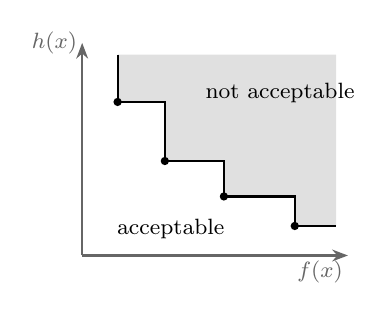
\begin{tikzpicture}[scale=0.75]
        \fill[black!12] (0.6,3.4)--(0.6,2.6)--(1.4,2.6)--(1.4,1.6)--(2.4,1.6)--(2.4,1.0)--(3.6,1.0)--(3.6,0.5)--(4.3,0.5)--(4.3,3.4)--cycle;
        \draw[thick] (0.6,3.4)--(0.6,2.6)--(1.4,2.6)--(1.4,1.6)--(2.4,1.6)--(2.4,1.0)--(3.6,1.0)--(3.6,0.5)--(4.3,0.5);
        \draw[vec,black!60] (0,0)--(4.5,0) node[lab,below left]{$f(x)$};
        \draw[vec,black!60] (0,0)--(0,3.6) node[lab,left]{$h(x)$};
        \foreach \p in {(0.6,2.6),(1.4,1.6),(2.4,1.0),(3.6,0.5)} \fill \p circle (2pt);
        \node[lab] at (3.35,2.75) {not acceptable};
        \node[lab] at (1.5,0.45) {acceptable};
      \end{tikzpicture}\\[0.2em]
      {\small Four pairs in a filter (Figure 15.6, redrawn).}
    \end{column}
  \end{columns}
  An accepted pair is added; pairs it dominates are removed. \readbook{pp.~437--439.}
\end{frame}

\begin{frame}{Feasibility restoration phase \from{Chapter 15}}
  \begin{itemize}\setlength\itemsep{0.4em}
    \item Problem with the filter: a line search may need arbitrarily small $\alpha_{k}$ before the trial point
      becomes acceptable. The algorithm stalls.
    \item Rule: if backtracking gives $\alpha_{k}<\alpha_{\min}$ (a threshold), switch to the
      \textbf{feasibility restoration phase}.
    \item The restoration phase ignores $f$ and only reduces the constraint violation:
      it approximately solves $\min_{x}h(x)$. $h$ is not smooth; Chapter 17 rewrites this as a smooth problem.
    \item It ends at a point with small $h$ that is acceptable to the filter.
    \item If $\min h(x)>0$ near the current point, the restoration phase converges to an infeasible point
      that locally minimizes the violation. A local method cannot always find a feasible point
      without a good starting point (p.~590).
  \end{itemize}
  \readbook{pp.~439--440.}
\end{frame}

\begin{frame}{Merit function and filter for the barrier problem}
  Both tests use the barrier function $f(x)-\mu\sum_{i}\log s_{i}$ of (19.4) in place of $f$:
  \[ \phi_{\nu}(x,s)=f(x)-\mu\sum_{i=1}^{m}\log s_{i}+\nu\|c_{\cE}(x)\|+\nu\|c_{\cI}(x)-s\| , \tag{19.26} \]
  $\ell_{1}$ or $\ell_{2}$ norm, not squared. $\nu$ is increased until $p$ is a descent direction for $\phi_{\nu}$ (p.~542).
  \begin{itemize}\setlength\itemsep{0.05em}
    \item Backtracking: $\alpha_{s}\in(0,\alpha_{s}^{\max}]$, $\alpha_{z}\in(0,\alpha_{z}^{\max}]$ \eqn{19.27};
      update as (19.8) with $\alpha_{s}$, $\alpha_{z}$ \eqn{19.28}.
    \item Filter pairs: (barrier function, $\|(c_{\cE}(x),\,c_{\cI}(x)-s)\|$). A rejection may start the restoration phase.
    \item Quasi-Newton: $\hessL$ replaced by BFGS, SR1 or L-BFGS (19.29). $s_{k}^{T}y_{k}>0$ is not guaranteed;
      damped BFGS (p.~537) modifies $y_{k}$ to keep $B_{k}$ positive definite.
  \end{itemize}
  \readbook{pp.~575--576.}
\end{frame}

\begin{frame}{Algorithm 19.2 (Line Search Interior-Point Algorithm)}
  \begin{block}{Algorithm 19.2}\small
    Choose $x_{0}$, $s_{0}>0$, $y_{0}$, $z_{0}>0$, $\mu>0$, $\eta,\sigma\in(0,1)$, $\epsilon_{\mu}$, $\epsilon_{\rm TOL}$; $k\la 0$.\\
    \textbf{repeat} until $E(x_{k},s_{k},y_{k},z_{k};0)\le\epsilon_{\rm TOL}$\\
    \quad\textbf{repeat} until $E(x_{k},s_{k},y_{k},z_{k};\mu)\le\epsilon_{\mu}$\\
    \qquad Compute $p=(p_{x},p_{s},p_{y},p_{z})$ from (19.12), modified as in (19.25) if necessary;\\
    \qquad Compute $\alpha_{s}^{\max}$, $\alpha_{z}^{\max}$ using (19.9); set $p_{w}=(p_{x},p_{s})$;\\
    \qquad Compute $\alpha_{s}$, $\alpha_{z}$ satisfying both (19.27) and\\
    \qquad\qquad $\phi_{\nu}(x_{k}+\alpha_{s}p_{x},s_{k}+\alpha_{s}p_{s})\le\phi_{\nu}(x_{k},s_{k})+\eta\alpha_{s}D\phi_{\nu}(x_{k},s_{k};p_{w})$;\\
    \qquad Compute $(x_{k+1},s_{k+1},y_{k+1},z_{k+1})$ using (19.28); update $B_{k}$ ($B_{0}\succ 0$) if quasi-Newton;\\
    \qquad Set $k\la k+1$;\\
    \quad\textbf{end};\quad Set $\mu\la\sigma\mu$ and update $\epsilon_{\mu}$;\\
    \textbf{end}\hfill\readbook{p.~577.}
  \end{block}
\end{frame}

\begin{frame}{Maratos effect: Example 15.4 \from{Chapter 15}}
  \begin{columns}[T,totalwidth=\textwidth]
    \begin{column}{0.66\textwidth}
      \[ \min\ 2(x_{1}^{2}+x_{2}^{2}-1)-x_{1}\ \ \text{s.t.}\ \ x_{1}^{2}+x_{2}^{2}-1=0 \tag{15.34} \]
      $\xs=(1,0)^{T}$, $\lambda^{*}=\tfrac32$, $\hessL(\xs,\lambda^{*})=I$.\\[0.1em]
      At the feasible point $x_{k}=(\cos\theta,\sin\theta)^{T}$, consider the step
      $p_{k}=(\sin^{2}\theta,\,-\sin\theta\cos\theta)^{T}$ \eqn{15.35}.
    \end{column}
    \begin{column}{0.32\textwidth}
      \centering
      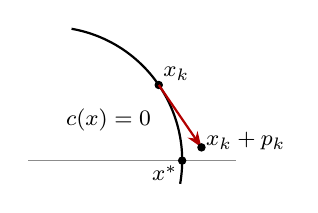
\begin{tikzpicture}[scale=1.7]
        \draw[black!45] (-0.15,0)--(1.4,0);
        \draw[thick] (0,0) ++(-10:1) arc (-10:80:1);
        \fill (1,0) circle (0.9pt) node[lab,below left]{$\xs$};
        \fill ({cos(34.4)},{sin(34.4)}) circle (0.9pt) node[lab,above right]{$x_{k}$};
        \draw[vec,red!70!black] ({cos(34.4)},{sin(34.4)})--({cos(34.4)+sin(34.4)^2},{sin(34.4)*(1-cos(34.4))});
        \fill ({cos(34.4)+sin(34.4)^2},{sin(34.4)*(1-cos(34.4))}) circle (0.9pt);
        \node[lab,right] at ({cos(34.4)+sin(34.4)^2},{sin(34.4)*(1-cos(34.4))+0.05}) {$x_{k}+p_{k}$};
        \node[lab] at (0.45,0.3) {$c(x)=0$};
      \end{tikzpicture}\\
      {\small $\theta=0.6$ (Figure 15.8, redrawn).}
    \end{column}
  \end{columns}
  \begin{itemize}\setlength\itemsep{0.3em}
    \item The step is good: $\|x_{k}+p_{k}-\xs\|_{2}\,/\,\|x_{k}-\xs\|_{2}^{2}=\tfrac12$, as in quadratic convergence.
    \item But $f(x_{k}+p_{k})=\sin^{2}\theta-\cos\theta>-\cos\theta=f(x_{k})$ and
      $c(x_{k}+p_{k})=\sin^{2}\theta>0=c(x_{k})$, for every $\theta\ne 0$.
    \item Every merit function $f+\mu h$ and the filter reject this step: the \textbf{Maratos effect}.
  \end{itemize}
  \readbook{pp.~440--442.}
\end{frame}

\begin{frame}{Second-order correction \from{Chapter 15}}
  Constraints as equalities $c(x)=0$ (here: $c_{\cE}(x)=0$, $c_{\cI}(x)-s=0$), with Jacobian $A_{k}$ at $x_{k}$.
  The step satisfies $A_{k}p_{k}+c(x_{k})=0$, but $c(x_{k}+p_{k})\ne 0$. Correct with
  \[ \hat p_{k}=-A_{k}^{T}(A_{k}A_{k}^{T})^{-1}c(x_{k}+p_{k}) , \tag{15.36} \]
  the minimum-norm solution of $A_{k}\hat p_{k}+c(x_{k}+p_{k})=0$.
  \begin{itemize}\setlength\itemsep{0.3em}
    \item Then $\|c(x_{k}+p_{k}+\hat p_{k})\|=O(\|x_{k}-\xs\|^{3})$, so near $\xs$ the corrected point decreases the
      merit function.
    \item Algorithm 15.2: if $\alpha=1$ fails the test (15.29), try $x_{k}+p_{k}+\hat p_{k}$. If that also fails,
      discard $\hat p_{k}$ and backtrack along $p_{k}$.
    \item Cost: one more evaluation of $c$ and one more solve with the factored matrix.
    \item Alternative: \textbf{watchdog} (Algorithm 15.3) lets the merit function increase on one step.
  \end{itemize}
  \readbook{pp.~443--445.}
\end{frame}

\section{\S19.7--19.8 Global and local behavior}

\begin{frame}{Example 19.2: the line search approach can fail}
  \begin{columns}[T,totalwidth=\textwidth]
    \begin{column}{0.56\textwidth}
      $\min x$\ \ s.t.\ $x^{2}-s_{1}-1=0$, $x-s_{2}-\tfrac12=0$, $s_{1},s_{2}\ge 0$ \eqn{19.53}.\\[0.2em]
      Feasible: $x\ge 1$. Start: left of the parabola, $s_{1}>0$.
      \begin{itemize}\setlength\itemsep{0.2em}
        \item A full step satisfies the linearized constraints: it ends on the tangent at $x^{(0)}$.
        \item (19.9) keeps $s_{1}>0$: the new point lies between the start and the tangent.
        \item The iterates stay in $\{x^{2}-s_{1}-1\ge 0,\ s_{1}\ge 0\}$ \eqn{19.54}.
      \end{itemize}
    \end{column}
    \begin{column}{0.42\textwidth}
      \centering
      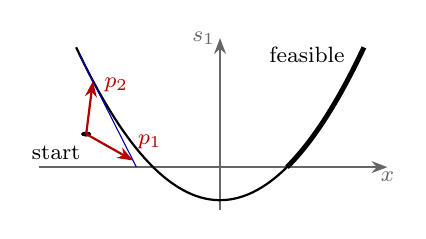
\begin{tikzpicture}[xscale=0.85,yscale=0.42]
        \draw[vec,black!60] (-2.7,0)--(2.5,0) node[lab,below]{$x$};
        \draw[vec,black!60] (0,-1.3)--(0,3.9) node[lab,left]{$s_{1}$};
        \draw[thick,domain=-2.15:1,samples=50] plot (\x,{\x*\x-1});
        \draw[line width=1.8pt,black,domain=1:2.15,samples=30] plot (\x,{\x*\x-1});
        \draw[blue!70!black,domain=-2.1:-1.25] plot (\x,{-4*\x-5});
        \fill (-2,1) circle (2.2pt);
        \node[lab] at (-2.45,0.45) {start};
        \draw[vec,red!70!black] (-2,1)--(-1.3,0.2);
        \node[lab,red!70!black] at (-1.05,0.75) {$p_{1}$};
        \draw[vec,red!70!black] (-2,1)--(-1.9,2.6);
        \node[lab,red!70!black] at (-1.55,2.5) {$p_{2}$};
        \node[lab,black] at (1.3,3.4) {feasible};
      \end{tikzpicture}\\
      {\small $x$--$s_{1}$ plane (Figure 19.2, redrawn). Blue: tangent at the start. Thick: feasible.}
    \end{column}
  \end{columns}
  \vspace{0.2em}
  Codes converge to $(-\beta,0,0)$, $\beta>0$: infeasible. No merit function or $\mu$ rule helps.
  Remedy: if $\alpha_{s},\alpha_{z}$ become very small, call the restoration phase. \readbook{pp.~587--589.}
\end{frame}

\begin{frame}{Fast local convergence}
  Near a solution with LICQ, strict complementarity and the second-order sufficient conditions
  (Assumptions 19.1), the full step $p$ of (19.12) is taken: careful implementations (with second-order
  correction) make the merit function or filter inactive there.
  \begin{itemize}\setlength\itemsep{0.3em}
    \item Goal: after one Newton step, $\alpha_{s}^{\max}=\alpha_{z}^{\max}=1$ and the inner test already holds for
      the next $\mu$. With $\epsilon_{\mu}=\theta\mu$ \eqn{19.57}, this is achieved by
      \[ \mu^{+}=\mu^{1+\delta},\quad\delta\in(0,1);\qquad\tau=1-\mu^{\beta},\quad\beta>\delta . \tag{19.58} \]
    \item Then the iterates converge superlinearly. With constant $\tau$ and $\mu^{+}=\sigma\mu$, the convergence is
      only linear. Decreasing $\mu$ faster than quadratically is useless.
    \item In practice the superlinear rate shows only in the last few iterations.
  \end{itemize}
  $\delta$, $\beta$, $\theta$ on this slide are the symbols of \S19.8, not those of (19.25) and (15.33).
  \readbook{pp.~591--592.}
\end{frame}

\section{IPOPT}

\begin{frame}{IPOPT and this chapter {\normalfont\small(Not in the book.)}}
  Sources: Wächter and Biegler, \emph{Math.\ Programming} 106 (2006), the book's reference [301]; IPOPT documentation.
  \begin{itemize}\setlength\itemsep{0.3em}
    \item Problem: $\min f(x)$ s.t.\ $c(x)=0$, $x_{L}\le x\le x_{U}$; general inequalities get internal
      slacks, as in (19.1). The Lagrangian is $f(x)+c(x)^{T}\lambda$ plus bound terms: the sign of $\lambda$ is
      opposite to (19.7).
    \item Linear system: the form (19.16). The inequalities are bounds, so $\Ai^{T}\Sigma\Ai$ is a diagonal
      matrix added to the Hessian. Required inertia: $(n,m,0)$, with $n$ variables (slacks included) and
      $m$ equality constraints.
    \item Globalization: line search with a filter, second-order corrections, restoration phase.
    \item Restoration phase: minimizes the $\ell_{1}$ violation, with $p,n\ge 0$ and $c(x)-p+n=0$,
      plus a term keeping $x$ near its starting point.
  \end{itemize}
\end{frame}

\begin{frame}{IPOPT defaults and the book {\normalfont\small(Not in the book.)}}
  \begin{center}\small\setlength\tabcolsep{5pt}
  \renewcommand{\arraystretch}{1.1}
  \begin{tabular}{lll}
    \toprule
     & IPOPT default & In the book \\
    \midrule
    $\mu$ & $\mu_{0}=0.1$; $\mu^{+}=\min\{0.2\mu,\,\mu^{1.5}\}$, at least $\epsilon_{\rm tol}/10$ & (19.18) and (19.58) \\
    Inner test & $E\le 10\,\mu$ & $E\le\mu$ in Alg.\ 19.1 \\
    $\tau$ & $\max\{0.99,\,1-\mu\}$ & (19.9); (19.58) \\
    $\delta_{w}$ & first trial $10^{-4}$, or $\tfrac13$ of the last one used & $\delta$ in (19.25), Alg.\ B.1 \\
    $\delta_{c}$ & $10^{-8}\mu^{1/4}$ if singular & $\gamma$ in (19.25), Alg.\ B.1 \\
    SOC & up to 4 per iteration & (15.36), Alg.\ 15.2 \\
    Hessian & exact; option: limited-memory & $\hessL$; option: (19.29) \\
    Stopping & $E(\cdot\,;0)\le 10^{-8}$, scaled & $E(\cdot\,;0)\le\epsilon_{\rm TOL}$ \\
    \bottomrule
  \end{tabular}
  \end{center}
  $\delta_{w}$ grows by a factor $100$ while no $\delta_{w}$ has been used before, by $8$ afterwards.\\
  Default \texttt{mu\_strategy} is \texttt{monotone}; \texttt{adaptive} updates $\mu$ at every iteration.
\end{frame}

\begin{frame}{Reading the IPOPT log: the columns {\normalfont\small(Not in the book.)}}
  \begin{center}\small\setlength\tabcolsep{5pt}
  \renewcommand{\arraystretch}{1.12}
  \begin{tabular}{lll}
    \toprule
    Column & IPOPT documentation & In this deck \\
    \midrule
    \texttt{iter} & iteration; \texttt{r} appended in restoration & $k$ \\
    \texttt{objective} & unscaled $f(x)$ & $f$ \\
    \texttt{inf\_pr} & max-norm of constraint violation & $\|c_{\cE}\|_{\infty}$, $\|c_{\cI}-s\|_{\infty}$ \\
    \texttt{inf\_du} & scaled max dual infeasibility & $\|\nabla f-\Ae^{T}y-\Ai^{T}z\|_{\infty}$ \\
    \texttt{lg(mu)} & $\log_{10}\mu$ & barrier parameter \\
    \texttt{||d||} & max-norm of primal step & $\|(p_{x},p_{s})\|_{\infty}$ \\
    \texttt{lg(rg)} & $\log_{10}\delta_{w}$; \texttt{-} if none & $\delta$ in (19.25) \\
    \texttt{alpha\_du}, \texttt{alpha\_pr} & dual, primal step sizes & $\alpha_{z}$, $\alpha_{s}$ \\
    \texttt{ls} & backtracking steps (without SOC) & line search \\
    \bottomrule
  \end{tabular}
  \end{center}
  \texttt{lg(mu)} constant for several lines, then a drop: the inner loop of Algorithm 19.2.\\
  \texttt{lg(rg)} not \texttt{-}: the inertia condition (19.24) failed and $\delta>0$ was added.
\end{frame}

\begin{frame}{Reading the IPOPT log: letters and exit messages {\normalfont\small(Not in the book.)}}
  Letter after \texttt{alpha\_pr}:
  \begin{itemize}\setlength\itemsep{0.25em}
    \item \texttt{h}: accepted by the filter test (15.33); \texttt{f}: accepted by an Armijo decrease of the
      barrier function, used when the constraint violation is already small.
      \texttt{H}, \texttt{F}: the same, with a second-order correction.
    \item \texttt{R}: restoration phase started; \texttt{w}: watchdog (Algorithm 15.3).
  \end{itemize}
  Exit messages:
  \begin{itemize}\setlength\itemsep{0.25em}
    \item \texttt{Optimal Solution Found}: $E(\cdot\,;0)\le$ \texttt{tol}. A KKT point, not a certified local
      or global solution.
    \item \texttt{Converged to a point of local infeasibility}: restoration reached a local minimizer of the
      violation that is infeasible.
    \item \texttt{Restoration Failed!}: no point acceptable to the filter was found.
    \item \texttt{Error in step computation!}: often the regularization became too large.
  \end{itemize}
\end{frame}

\section{Chapters not covered}

\begin{frame}{Chapters not covered, and where they appear in IPOPT}
  \begin{center}\small\setlength\tabcolsep{6pt}
  \renewcommand{\arraystretch}{1.2}
  \begin{tabular}{lll}
    \toprule
    Chapter & Content & Where it appears \\
    \midrule
    8, 9 & derivatives (AD); derivative-free & IPOPT needs $\nabla f$, $\nabla c_{i}$, $\hessL$ \\
    10, 11 & least squares; nonlinear equations & (19.2) is a nonlinear equation \\
    13, 14 & simplex; interior-point for LP & predictor rule (19.21) \\
    15 & merit, filter, Maratos, SOC & in this deck \\
    16 & QP, KKT matrix, inertia & Theorem 16.3, (16.12) \\
    17 & $\ell_{1}$ penalty, augmented Lagrangian & IPOPT restoration problem \\
    18 & SQP, damped BFGS & the alternative to interior-point \\
    \bottomrule
  \end{tabular}
  \end{center}
  SQP solves a QP at each step; the active set of the QP estimates the optimal active set. Interior-point
  methods are often faster on large problems, but every step involves all constraints (pp.~592--593).
  Not covered: \S19.5, \S19.6.
\end{frame}

\section{Homework}

\begin{frame}{Homework {\normalfont\small(problem 4 is not in the book)}}
  \begin{enumerate}\setlength\itemsep{0.25em}
    \item Exercise 19.1(a): match the KKT points of (19.1) with those of
      $\min f(x)$ s.t.\ $c_{\cE}(x)=0$, $c_{\cI}(x)\ge 0$.
    \item Exercise 19.5(b): as $\mu\to 0$, which diagonal elements of $\Sigma$ tend to $\infty$ and which to $0$?
      Answer for $\Sigma=S^{-1}Z$ and for $\Sigma=\mu S^{-2}$.
    \item Exercise 19.12(c): $\min x$ s.t.\ $x\ge 0$, $1-x\ge 0$. Find the minimizer $x(\mu)$ of
      $P(x;\mu)=x-\mu\log x-\mu\log(1-x)$ and its limit as $\mu\to 0$.
    \item $G=\mathrm{diag}(1,-1)$, $A=[1\ \ 0]$, $K(\delta)=\begin{bmatrix} G+\delta I & A^{T}\\ A & 0\end{bmatrix}$.
      (a) Find the inertia of $K(0)$ and all $\delta\ge 0$ with inertia $(2,1,0)$; check with Theorem 16.3.
      (b) Which $\delta$ does Algorithm B.1 return, starting from $\delta_{\rm old}=0$?
    \item Exercise 19.11(c): problem (19.53) with $x^{(0)}=-2$, $s^{(0)}=(1,1)$, $z^{(0)}=(1,1)$, $\mu=0$.
      Compute the Newton step of (19.6), truncate it with (19.9) and $\tau=1$, and check that the new
      iterate is in the region (19.54).
  \end{enumerate}
\end{frame}

\end{document}
